% \documentclass[usenames,dvipsnames,notes]{beamer}
\documentclass[usenames,dvipsnames]{beamer}

\usetheme{uhh}
\showtotalframenumber
\showuhhlogoeachframe
\showsections

\usepackage{ textcomp }
\usepackage{booktabs}
\usepackage{xcolor}
\usepackage{amsmath}
\usepackage{graphicx}
\usepackage{tabularx}
\usepackage{color}
\DeclareMathOperator*{\argmin}{arg\,min}

\usepackage{listings}
\lstset{
  language=python
  }



\DeclareMathOperator{\tf}{tf}
\DeclareMathOperator{\tfidf}{tf-idf}
\DeclareMathOperator{\coverage}{coverage}
\DeclareMathOperator{\dist}{dist}
\DeclareMathOperator{\SPD}{SPD}
\DeclareMathOperator{\pscore}{\mathit{p}-score}
\DeclareMathOperator{\gold}{gold}
\DeclareMathOperator{\LCH}{LCH}
\DeclareMathOperator{\hscore}{\mathit{h}-score}
\DeclareMathOperator{\hpcscore}{\mathit{hpc}-score}
\DeclareMathOperator{\hpcavg}{\mathit{hpc}-avg}
\DeclareMathOperator{\cbadnessval}{\mathit{c}-badness}
\DeclareMathOperator{\hbadnessval}{\mathit{h}-badness}
\DeclareMathOperator{\badnessval}{badness}
\DeclareMathOperator{\pvalue}{\mathit{p}-value}



\title{Improving Hypernymy Extraction with Distributional Semantic Classes}

\author[Panchenko et al. LREC'18]{\underline{Alexander Panchenko}, Dmitry Ustalov, Stefano Faralli, Simone Paolo Ponzetto, and Chris Biemann}
% \institute{$^1$ University of Hamburg, Department of Informatics, Language Technology Group, Germany \\
%         $^2$ University of Mannheim, School of Business Informatics and Mathematics, Data and Web Science Group} 
\date[10.05.2018]{May 10, 2018}

\AtBeginSection[]
{
   %%%%% section title
   % This is how it would look like in Beamer:
   % \begin{frame}
   %     \frametitle{Overview}
   %     \tableofcontents[sections={2-3},currentsection,sectionstyle=show/hide,subsectionstyle=hide]
   % \end{frame}
  \begin{frame}[plain]
  \begin{tikzpicture}[overlay]
    \relax%
    \fill[blueuhh,opacity=1] (-10,-10)
    rectangle(\the\paperwidth,\the\paperheight);
  \end{tikzpicture}
   \begin{tikzpicture}[overlay]
    \relax%
    \fill[white,opacity=1] (-5,-1.2)
    rectangle(\the\paperwidth,0.5) node[pos=0.5,black]{\LARGE\insertsectionhead};
  \end{tikzpicture}
  \end{frame}

  %%%% add subsection to show navigation dots
  \subsection{}
}


\begin{document}

\maketitle

%
\section{Overview}

\begin{frame}
  \frametitle{Overview}

  \begin{itemize}
		\item \alert{\textbf{Inducing word sense representations}}:
		\begin{itemize}
		\item \textbf{word sense embeddings via retrofitting} \cite{pelevina-EtAl:2016:RepL4NLP,remus:2018};
		\item \textbf{inducing synsets}~\cite{ustalov-panchenko-biemann:2017:Long,ustalov2017fighting,madoc43362}
		\item \textbf{inducing semantic classes} \cite{panchenko:2018:SemanticClasses} 
		\end{itemize}
	
	
	
	\pause 
	\vspace{1em}
	\item \alert{\textbf{Making induced senses interpretable}} \cite{panchenko-EtAl:2017:EMNLP2017Demos,panchenko-EtAl:2017:EACLlong}
	
	\pause
	\vspace{1em}
	\item \alert{\textbf{Linking induced word senses to lexical resources}}~\cite{panchenko2016best,faralli2016linked,panchenko-EtAl:2017:SENSE2017,biemann2018framework}	
			
\end{itemize}
	
\end{frame}

\section{Introduction}
\subsection{}


\begin{frame}{Hypernyms}

\begin{block}{Examples of hypernymy relations}
\begin{itemize}
	\item \textbf{apple} --isa\textrightarrow \textbf{ fruit}
	\item \textbf{mangosteen} --isa\textrightarrow \textbf{ fruit}
\end{itemize}
\end{block}

\vspace{92pt}

$ $ 
\end{frame}


\begin{frame}{Hypernyms}

\begin{block}{Examples of hypernymy relations}
\begin{itemize}
	\item \textbf{apple\alert{\#1}} --isa\textrightarrow \textbf{ fruit\alert{\#2}}
	\item \textbf{mangosteen\alert{\#0}} --isa\textrightarrow \textbf{ fruit\alert{\#2}}
\end{itemize}
\end{block}

\pause

``\textbf{This caf\'e serves fresh \alert{\underline{mangosteen}} juice}''

\pause 

\begin{block}{Examples of applications of hypernyms}
\begin{itemize}
	\item question answering~\cite{Zhou:13} 
	\item query expansion~\cite{gong2005web}
	\item semantic role labelling~\cite{shi2005putting} 
\end{itemize}
\end{block}


\note{Hypernyms are also the building blocks for learning taxonomies from text~\cite{bordea2016semeval}. Consider the following sentence: . Here the infrequent word ``mangosteen'' may be poorly represented or even absent in the vocabulary of a statistical model, yet it can be substituted by lexical items with better representations, which carry close meaning, such as its hypernym ``fruit'' or one of its close co-hyponyms, e.g. ``mango''. }

\end{frame}


\begin{frame}{Automatic extraction of hypernyms}

\vspace{-10pt}
\begin{block}{A short history of extraction methods}
\begin{enumerate}
	\item \cite{hearst1992automatic}: lexical-syntactic patterns \textbf{\alert{defined manually}};

	\pause 
		
	\item \cite{snow2004learning}: lexical-syntactic patterns learned in \textbf{\alert{a supervised way}};
	
	\pause 
	
	\item \cite{weeds2014learning}: supervised approach with \textbf{\alert{word embedding features}};
	
	\item \cite{shwartz-goldberg-dagan:2016:P16-1}: supervised approach with \textbf{\alert{word and path embedding features}};
	
	\item \cite{glavavs-ponzetto:2017:EMNLP2017,ustalov-EtAl:2017:EACLshort}: taking into account \textbf{\alert{assymetry}} of hypernyms.

\end{enumerate}
\end{block}

\pause 

\textbf{Not taking into account \alert{word senses} and \alert{global structure}!}

 \note{Frequencies of the extracted relations usually follow a power-law, with a long tail of noisy extractions containing rare words. We propose a method that performs post-processing of such noisy binary hypernyms using distributional semantics, cf. Figure~\ref{fig:cosetbinary}. Namely, we use the observation that distributionally related words are often are co-hyponyms~\cite{wandmacher2005semantic,Heylen:08} and operationalize it to perform filtering of noisy relations by finding dense graphs composed of both hypernyms and co-hyponyms.  }
 
\end{frame}



\begin{frame}{Induction of semantic classes}

``\textbf{\alert{Global distributional structure}}'' of a language $\approx$ global sense clustering, e.g. {\footnotesize \underline{\url{panchenko.me/data/joint/nodes20000-layers7}}}

\vspace{-5pt}
\begin{center}
\includegraphics[width=.7\textwidth]{figures/structure}
\end{center}

\end{frame}



\begin{frame}{Induction of semantic classes}

``\textbf{\alert{Global distributional structure}}'' of a language $\approx$ global sense clustering, e.g. {\footnotesize \underline{\url{panchenko.me/data/joint/nodes20000-layers7}}}

\vspace{-5pt}
\begin{center}
\includegraphics[width=.65\textwidth]{figures/structure1.png}
\end{center}

\end{frame}


\begin{frame}{Induction of semantic classes}

\begin{block}{A short history of extraction methods}

\begin{enumerate}
	\item  \cite{Lin2001}: sets of similar words are clustered into concepts.
	\item \cite{Pantel2002}: words can belong to several clusters (representing senses)
	\item \cite{Pantel2004}: aggregate hypernyms per cluster from from Hearst patterns
 

\end{enumerate}
\end{block}

\textbf{No explicit evaluation of \alert{usefulness} of hypernymy labels for \alert{hypernymy extraction}.}

\end{frame}

\begin{frame}{Main contributions}

\note{The contribution of the paper is an unsupervised method for post-processing of noisy hypernymy relations based on  clustering of graphs of word senses induced from text. The idea to use distributional semantics to find hypernyms seems natural and has been widely used. However, the existing methods used distributional, yet \textit{sense-unaware} and \textit{local} features. We are the first to use \textit{global sense-aware distributional structure} via the induced semantic classes to improve hypernymy extraction. The implementation of our method and the induced language resources (distributional semantic classes and cleansed hypernymy relations) are available online.}

\begin{itemize}
	\item We show how distributionally-induced \alert{\textbf{semantic classes}} can be helpful  for \alert{\textbf{extracting hypernyms}}:
	\pause
	\vspace{10pt}
	\begin{enumerate}
		\item A method for \textbf{\alert{inducing sense-aware semantic classes}} using distributional semantics; 
		\vspace{10pt}
		\item A method for using the induced semantic classes for \textbf{\alert{filtering noisy hypernymy relations}}.
	 \end{enumerate}
\end{itemize}
\end{frame}

\section{Method}
\subsection{}


\begin{frame}{ Labeled semantic classes}

\begin{figure}[ht]
  \centering
  \includegraphics[width=.99\textwidth]{figures/coset}

\end{figure}

\begin{itemize}
\item \textbf{\alert{Post-processing of hypernymy relations}} using distributionally induced semantic classes;
\item A semantic class is a clusters of induced word senses \textbf{\alert{labeled with hypernyms}}.

\end{itemize}

\note{The word postfix, such as \texttt{\#1}, is an ID of an induced sense. The wrong hypernyms outside the cluster labels are removed, while the missing ones not present in the noisy database of hypernyms are added. }


\end{frame}


\begin{frame}{Outline of our approach}



\begin{enumerate}
	\item Sense-aware distributional semantic classes are \textbf{induced from a text corpus}; 
	\item Semantic classes are used to \textbf{filter a noisy hypernyms} database. 
 
\end{enumerate}

\pause 


\begin{figure}
  \centering
  \includegraphics[width=.99\textwidth]{figures/outline}
  \end{figure}


\note{(e.g. extracted by an external method from a text corpus)}

\end{frame}


\begin{frame}[fragile]
\frametitle{Chinese Whispers\#1}
\begin{center}
 \includegraphics[height=0.52\textwidth]{figures/cw}
 
  {\tiny * source of the image: \url{http://ic.pics.livejournal.com/blagin_anton/33716210/2701748/2701748_800.jpg}}
 \end{center}
\end{frame}



\begin{frame}[fragile]
\frametitle{Chinese Whispers\#2: \alert{graph clustering}}
\begin{center}
 \includegraphics[height=0.59\textwidth]{figures/cw2-1}
 
  %{\tiny * source of the image: [Biemann, 2006]}
 \end{center}
\end{frame}


\begin{frame}[fragile]
\frametitle{Chinese Whispers\#2: \alert{graph clustering}}
\begin{center}
 \includegraphics[height=0.59\textwidth]{figures/cw2-2}
 
  %{\tiny * source of the image: [Biemann, 2006]}
 \end{center}
\end{frame}

\begin{frame}[fragile]
\frametitle{Chinese Whispers\#2: \alert{graph clustering}}
\begin{center}
 \includegraphics[height=0.59\textwidth]{figures/cw2}
 
  %{\tiny * source of the image: [Biemann, 2006]}
 \end{center}
\end{frame}


\begin{frame}{Graph-based word sense induction}

\note{Word sense induction using  ego-network clustering. We also use such CW clustering for the global clustering as well. }

	
\centering
\begin{figure}
\includegraphics[width=0.9\textwidth]{figures/table}
\end{figure}

\end{frame}

	
\begin{frame}{Sample of induced sense inventory}


\begin{table}
\centering
\scriptsize
\begin{tabular}{l|p{6cm}|p{2.5cm}} 
\bf Word Sense & \bf Local Sense Cluster: Related Senses & \bf Hypernyms \\
\toprule
 \alert{mango\#0} &  peach\#1, grape\#0, plum\#0, apple\#0, apricot\#0, watermelon\#1, banana\#1, coconut\#0, pear\#0, fig\#0, melon\#0,  \alert{\textbf{mangosteen\#0}}, ... & fruit\#0, food\#0, ... \\
 
\midrule
\alert{apple\#0} & mango\#0, pineapple\#0, banana\#1, melon\#0, grape\#0, peach\#1, watermelon\#1, apricot\#0, cranberry\#0, pumpkin\#0, \alert{\textbf{mangosteen\#0}}, ... & fruit\#0, crop\#0,  ... \\

\midrule
Java\#1 & C\#4, Python\#3, Apache\#3, Ruby\#6, Flash\#1, C++\#0, SQL\#0, ASP\#2, Visual Basic\#1, CSS\#0, Delphi\#2, MySQL\#0, Excel\#0, Pascal\#0, ... & programming language\#3, language\#0, ... \\

\midrule
Python\#3 & PHP\#0, Pascal\#0, Java\#1, SQL\#0, Visual Basic\#1, C++\#0, JavaScript\#0, Apache\#3, Haskell\#5, .NET\#1, C\#4, SQL Server\#0, ... & language\#0, technology\#0, ... \\

\end{tabular}


\end{table}


\note{ entries  representing ``fruits'' and ``programming language'' senses. Each word sense $s$ is represented with a list of related senses $\mathcal{N}(s)$ and the list of hypernyms $\mathcal{H}(s)$. The hypernyms can be used as human-interpretable sense labels of the sense clusters. One sense $s$, such as ``apple\#0'', can appear in multiple entries.}

\end{frame}


\begin{frame}{Sample of induced  semantic classes}


\begin{table}
\centering
\scriptsize
\begin{tabular}{l|p{2.5in}|p{1in}} 
\bf ID &  \bf Global Sense Cluster: Semantic Class & \bf Hypernyms \\ 

\toprule

1 & peach\#1, banana\#1, pineapple\#0, berry\#0, blackberry\#0, grapefruit\#0, strawberry\#0, blueberry\#0, \alert{mango\#0}, grape\#0, melon\#0, orange\#0, pear\#0, plum\#0, raspberry\#0, watermelon\#0, \alert{apple\#0}, apricot\#0, watermelon\#0, pumpkin\#0, berry\#0, \alert{\textbf{mangosteen\#0}}, ...  & vegetable\#0, fruit\#0, crop\#0, ingredient\#0, food\#0, $\cdot$ \\ 

\midrule

2  & C\#4, Basic\#2, Haskell\#5, Flash\#1, \alert{Java\#1}, Pascal\#0, Ruby\#6, PHP\#0, Ada\#1, Oracle\#3, \alert{Python\#3}, Apache\#3, Visual Basic\#1, ASP\#2, Delphi\#2, SQL Server\#0, CSS\#0, AJAX\#0, JavaScript\#0, SQL Server\#0, Apache\#3, Delphi\#2, Haskell\#5, .NET\#1, CSS\#0, ... & programming language\#3, technology\#0, language\#0, format\#2, app\#0
\end{tabular}

\note{Sample of the induced  sense clusters representing ``fruits'' and ``programming language'' semantic classes. Similarly to the induced word senses, the semantic classes are labeled with hypernyms. In contrast to the induced word senses, which represent a local clustering of word senses (related to a given word) semantic classes represent a global sense clustering of word senses. One sense $c$, such as ``apple\#0'', can appear only in a single cluster.}


\end{table}

\end{frame}

%\begin{frame}{A non-coherent ego network}
%
%\begin{figure}
%  \centering
%  \includegraphics[width=.99\textwidth]{figures/ego-network}
%\end{figure}
%
%\note{An example of a non-coherent ego network  of the automatically induced sense \texttt{Python\#1}, representing the ``animal" sense. We prune it to remove terms not relevant to the animal sense. }
%  	
%\end{frame}

\begin{frame}{Network of induced word senses}
	
	
\begin{figure}[ht]
  \centering
  \includegraphics[width=.99\textwidth]{figures/cluster-programming}
\end{figure}

  \note{Senses referring to programming languages co-occur in global sense cluster entries, resulting in a densely connected set of co-hyponyms. }

\end{frame}

% extra slide ...

\section{Optimization of meta-parameters}
\subsection{}
\begin{frame}{Comparison to WordNet and BabelNet}

\begin{block}{Meta-parameters}	
\begin{enumerate}
\item \textbf{Min. num. of sense co-occurrences in an ego-network}: $t > 0$
\item \textbf{Sense edge weight type}: count or log(count) 
\item \textbf{Hypernym weight type}: tf-idf or tf
\end{enumerate}
\end{block}

\pause 

% & $\hpcavg$, \textbf{WordNet} & $\hpcavg$, \textbf{BabelNet

$$
  \hpcscore(c) = \frac{\hscore(c) + 1}{\pscore(c) + 1} \cdot \coverage(c)\text{.}
$$

$$
  \pscore(c) = \frac{1}{\left\vert{}c\right\vert} \sum^{\left\vert{}c\right\vert}_{i=1} \sum^i_{j=1} \dist(w_i, w_j)\text{.}
  \hscore(c) = \frac{\left\vert\mathcal{H}(c) \cap \gold(c)\right\vert}{\left\vert\mathcal{H}(c)\right\vert}\text{.}
$$
	
\note{
The method has really just a few parameters, but still we wanted to know their impact... 

Since we are in an unsupervised setting...

Performance of different configurations of the hypernymy labeled global sense clusters in terms of their similarity to WordNet/BabelNet. The results are sorted by performance on BabelNet dataset, the best values in each section are boldfaced. The two underlined configurations are respectively the best \textit{coarse-grained} and \textit{fine-grained} grained semantic class models used in all experiments. The coarse grained model contains less semantic classes, but they tend to be more consistent than those of the fine-grained model, which contains more senses and classes. }

	
\end{frame}


\begin{frame}{Impact of the min. edge weight $t$}

\begin{figure}
  \centering
  \includegraphics[width=.99\textwidth]{figures/t}
 \end{figure}
	
	\note{ The higher the threshold the better quality relations we get, ... but the smaller the network becomes}
  
\end{frame}



\begin{frame}{Best coarse- and fine-grained models}


\begin{table}
\scriptsize
\centering
\begin{tabular}{p{1.4cm}|p{1.2cm}|p{1.2cm}|p{1.3cm}|p{1.1cm}|p{1.2cm}|p{1.2cm}}
  \textbf{Min. num of sense co-occurr.}, $t$ & \textbf{Edge weight}, $E$ & \textbf{Hypernym weight}, $H$ & \textbf{Number of clusters} & \textbf{Number of senses} & $\hpcavg$, \textbf{WordNet} & $\hpcavg$, \textbf{BabelNet} \\ \toprule

0  & count  & tf-idf & \textbf{\alert{1\,870}} & \textbf{\alert{208\,871}} & 0.041 & 0.279 \\

100 & log  & tf-idf & \textbf{\alert{734}} &  \textbf{\alert{18\,028}} & 0.092 & 0.304 \\ \midrule

 
\end{tabular}

\end{table}

	
\end{frame}



\section{Results}
\subsection{Plausibility of Semantic Classes}

\begin{frame}{Plausibility of Semantic Classes}

\begin{columns}
\begin{column}{0.4\textwidth}

\includegraphics[width=1.0\textwidth]{figures/e1}

\pause

 \begin{itemize}
\item Layout of the sense cluster evaluation crowdsourcing task;
 
 \item the entry ``\textbf{\alert{winchester}}'' is the \textbf{intruder}.
\end{itemize}
\end{column}
\begin{column}{0.6\textwidth}  

\begin{figure}
  \centering
  \includegraphics[width=.99\textwidth]{figures/cluster-hit}
\end{figure}

\end{column}
\end{columns}




\note{Comparison to gold standard resources allows us to gauge the relative performances of various configurations of our method. To measure the absolute quality of the best configuration selected in the previous section, we rely on microtask-based crowdsourcing with CrowdFlower. 

We used two crowdsourcing tasks based on word intruder detection~\cite{Chang:09} to measure how humans perceive the extracted lexical-semantic structures. Namely, the tasks are designed to evaluate the quality of the extracted sense clusters and their labels. The input form presented to an annotator is illustrated in.

A crowdworker is asked to identify words that do not match the context represented by words from a sense cluster or its label. To generate an intruder, following the original design of~, we select a random word from a cluster and replace it with a word of similar frequency that does not belong to any cluster (bias here is low as the evaluated model contains 27,149 out of  313,841 induced word senses). In both tasks, the workers have been provided with concise instructions and test  questions. 

\textbf{Evaluation Metrics}

We compute two metrics on the basis on annotation results: (1) \textit{accuracy} is the fraction of tasks where annotators correctly identified the intruder, thus the words from the cluster are consistent; (2) \textit{badness} is the fraction of tasks for which non-intruder words were selected. In this experiment, we assume that it is easy to identify the intruder in a correct sense cluster and difficult in a noisy, implausible sense cluster. We compute \textit{accuracy} as the fraction of tasks where annotators correctly identified the intruder, thus the words from the cluster are consistent.
}

\end{frame}



\begin{frame}{Plausibility of Semantic Classes}

\note{Plausibility of the sense clusters according to human judgments via an intruder detection experiment for the coarse-grained semantic class model.}

\begin{enumerate}
	\item \textbf{Accuracy} is the fraction of tasks where annotators correctly identified the intruder; 
	\item \textbf{Badness}: is the fraction of tasks for which non-intruder words were selected.  
\end{enumerate}

\pause

\begin{tabular}{l|c|c|c}
\textbf{} & \textbf{Accuracy} & \textbf{Badness} & \textbf{Randolph $\kappa$} \\ \toprule
Sense clusters, $c$ & $0.859$ & $0.248$ & $0.739$ \\
Hyper. labels, $\mathcal{H}(c)$  & $0.919$ & $0.208$ & $0.705$ \\
\end{tabular}

\pause 

\begin{itemize}
	\item \textbf{Clusters}: 68 annotators, 2,035 judgments; 
	\item \textbf{Hypernyms}: 98 annotators, 2,245 judgments.
\end{itemize}

\end{frame}



\begin{frame}{ Improving Hypernymy Relations }

\vspace{-20pt}

\begin{center}
\includegraphics[width=0.5\textwidth]{figures/e2}
\end{center}

\pause

Layout of the hypernymy annotation task:

\begin{figure}
  \centering
  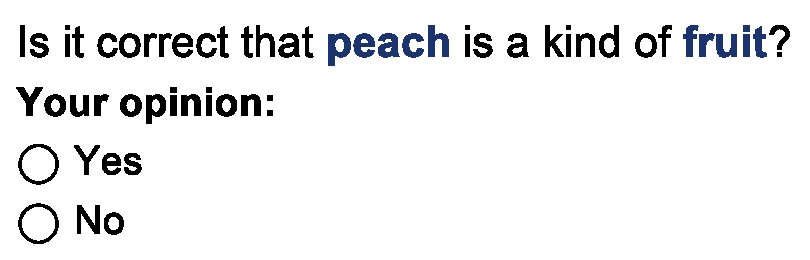
\includegraphics[width=.75\textwidth]{figures/exp3-hit}
\end{figure}

\end{frame}


\begin{frame}{ Improving Hypernymy Relations }

Evaluating results of post-processing of a noisy hypernymy database using human judgements:


\begin{itemize}
	\item A random sample of 4,870 relations using lexical split; 
	\item each labeled 6.9 times on average;
	\item a total of 33,719 judgments.
\end{itemize}

\pause 

\begin{table}
\footnotesize
\centering

\begin{tabular}{p{6cm}|c|c|c}
 & \textbf{Precision} & \textbf{Recall} & \textbf{F-score} \\ \toprule
\textbf{\alert{Original}} hypernymy relations extracted from Common Crawl corpus~\cite{seitner2016large} & $0.475$ & $0.546$ & $0.508$ \\ \midrule 
\textbf{\alert{Enhanced}} hypernyms with the \textit{coarse-grained} semantic classes   & $\mathbf{0.541}$ & $\mathbf{0.679}$ & $\mathbf{0.602}$ \\ 
\end{tabular}

\end{table}

\end{frame}


\begin{frame}{ Improving Taxonomy Induction }

\begin{itemize}
	\item \textbf{SemEval 2016 Task 13} "Taxonomy Extraction from Text";
	\item \textbf{Fowlkes\&Mallows Measure (F\&M)} -- a cumulative measure of the similarity of taxonomies;
	\item \textbf{English} part of the dataset.
\end{itemize}

\pause 


\note{Summary of the domain-specific sense clusters.}

\begin{table}
\footnotesize
\centering
\begin{tabular}{l|p{0.9cm}|p{1.4cm}|p{1.3cm}|p{1.5cm}}
\textbf{Domain} & \textbf{\#Seeds words} & \textbf{\#Expanded words} & \textbf{\#Clusters}, fine-gr. & \textbf{\#Clusters}, coarse-gr.  \\ \toprule
Food & 2\,834 & 3\,047 & 29 & 21 \\
Science & 806 & 1\,137 & 73 & 35 \\
Environ. & 261 & 909 & 111 & 39 \\
\end{tabular}
\end{table}


\end{frame}



\begin{frame}{ Improving Taxonomy Induction }


\begin{table}
\scriptsize
\centering
\begin{tabular}{p{2.6cm}|p{1cm}|p{1cm}|p{1cm}|p{1cm}|p{1cm}|p{1cm}}
\textbf{System / Dataset} & \textbf{Food, WordNet} & \textbf{Science, WordNet}& \textbf{Food, Combined} & \textbf{Science, Combined} & \textbf{Science, Eurovoc} & \textbf{Environ., Eurovoc} \\ \toprule

WordNet & 1.0000 & 1.0000 & 0.5870 & 0.5760 & 0.6243 & n.a. \\ \midrule

Baseline & 0.0022 & 0.0016 & 0.0019 & 0.0163 & 0.0056 & 0.0000 \\
JUNLP & 0.1925 & 0.0494 & 0.2608 & 0.1774 & 0.1373 & 0.0814 \\
NUIG-UNLP & n.a. & 0.0027 & n.a. & 0.0090 & 0.1517 & 0.0007 \\
QASSIT & n.a. & 0.2255 & n.a. & 0.5757 & 0.3893 & 0.4349 \\
TAXI & 0.3260 & 0.2255 & 0.2021 & 0.3634 & 0.3893 & 0.2384 \\
USAAR & 0.0021 & 0.0008 & 0.0000 & 0.0020 & 0.0023 & 0.0007 \\ \midrule

Sem. Class, fine-gr. & 0.4540 & 0.4181 & 0.5147 & 0.6359 &  \textbf{0.5831} & 0.5600 \\
Sem. Class, coarse-gr. & \textbf{0.4774} & \textbf{0.5927} & \textbf{0.5799} & \textbf{0.6539} & 0.5515 & \textbf{0.6326} 
\end{tabular}
\end{table}


\end{frame}



\begin{frame}{ Summary }

\begin{enumerate}
	\item An unsupervised method for the induction of \textbf{\alert{sense-aware distributional semantic classes}};
	\item Showed how these can be used for \textbf{\alert{post-processing of noisy hypernymy databases}} extracted from text.
\end{enumerate}

\note{By using global as opposed to local information ...}

\begin{center}
\includegraphics[width=.9\textwidth]{figures/coset}
\end{center}

\end{frame}

\begin{frame}{ $  $ }

{\Huge Thank you! Questions?}
\begin{center}
	\includegraphics[width=.7\textwidth]{figures/mangosteen}
\end{center}
\end{frame}

\bibliography{biblio}
\bibliographystyle{apalike2}


\end{document}

